\section{Thermal cameras}

Thermal cameras are transducers that convert infrared (IR) radiation into electrical signals, which can be used to form a thermal image.
IR is an electromagnetic (EM) radiation and covers part of EM spectrum that is invisible to the human eye.
IR spectrum covers wavelengths from 780 \si{\micro\meter} to 1 \si{\milli\meter}, but only small part of that spectrum is used for IR imaging ( from 0.9 \si{\micro\meter} to 14 \si{\micro\meter})\cite{thermal_book}.
We can broadly classify IR cameras into two categories: photon detectors or thermal detectors\cite{thermal_book}.
Photon detectors convert absorbed EM radiation directly into electric signals by the change of concentration of free charge carriers\cite{thermal_book}.
Thermal detectors, covert absorbed EM radiation into thermal energy, raising the detector temperature\cite{thermal_book}. 
Change of detector's temperature is then converted into an electrical signal.

Common examples of thermal detectors are thermopiles and microbolometers. 
Thermopiles are composed of several thermocouples.
Thermocouple consists of two different metals joined at one end, which is known as hot junction.
Other two ends of the metals are known as cold junctions.
When there is a temperature difference between the hot and cold junctions, voltage proportional to that difference is generated on open ends of the metals.
To increase voltage responsivity, several thermocouples are connected in series to form a thermopile\cite{thermal_book}.
Thermopiles have lower responsivity when compared to microbolometers, but they do not require temperature stabilization\cite{thermal_book}.

Thermal camera FLIR Lepton that we will use for this project is a microbolometer, so we will describe these types of detectors in greater detail.
Microbolometers can be found in most IR cameras today\cite{thermal_book}. 
They are sensitive to IR wavelengths of 8 to 14 \si{\micro\meter}, which is a part of longwave infrared region (LWIR)\cite{thermal_book}.
Measuring part of an microbolometer is known as focal point array (FPA) (Figure \ref{FPA}).
FPA consists of IR thermal detectors, bolometers (Figure \ref{FPA_pixel}), that can convert IR radiation into electric signal.
Each bolometer consists of an absorber material connected to an readout integrated circuit (ROIC) over thermally insulated, but electrically conductive legs\cite{thermal_article}.

\begin{figure}[h]
    \begin{subfigure}{0.5\textwidth}
        \centering
        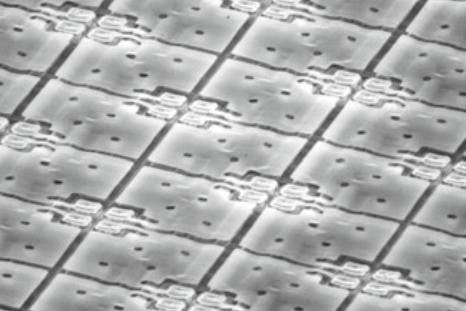
\includegraphics[width=1.0\linewidth, height=5cm]{FPA.png} 
        \caption{}
        \label{FPA}
    \end{subfigure}
    \begin{subfigure}{0.5\textwidth}
        \centering
        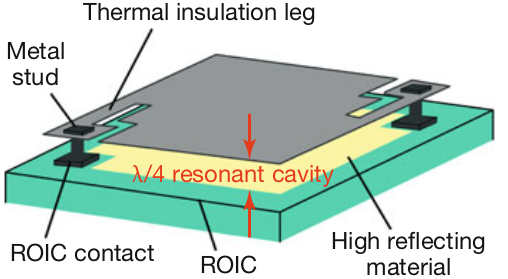
\includegraphics[width=1.0\linewidth, height=5cm]{FPA_pixel.png}
        \caption{}
        \label{FPA_pixel}
    \end{subfigure}

    \caption{(a) Focal point array under electronic microscope. (b) Bolometer with $\lambda /4$ resonant cavity. Image courtesy: Vollmer, Möllmann\cite{thermal_book}}
    \label{FPA_microbolo}
\end{figure}

Absorber material is made either out of metals such as gold, platinum, titanium or more commonly out of semiconductors such as vanadium-oxide (VOx)\cite{thermal_article}.
Important property of absorber materials is that electrical resistance changes proportionally with material's temperature\cite{thermal_book}.
When IR radiation hits absorber material, it is converted into thermal energy, which raises absorber's temperature, thus changing its resistance.
To detect change in resistance, ROIC applies steady-state bias current to absorber material, while measuring voltage over conductive legs\cite{thermal_book}. 





Oporne točke:
 - Kaj detektirajo termalne kamere
 - osnovna razdelitev na optične in termalne.
 - idi v podrbno v termalne, omeni thermopile in microbolometere, njihove lastnosti
 - povej zakaj se je Arribada odločila za flir
 - razloži osnovni princip delovanja microbolometera (slika)

Kako deluje microbolometer
https://www.sciencedirect.com/science/article/pii/S0961129006717641

    - Zakjaj boš uporabal določeno kamero, flir lepton, Kako deluje termalna kamera, na kakšen način lahko kamera spremni output, resolucija, refresh, zunanji vplivi

 2. Theoretical description of system building blocks
    Not sure what to write here, before starting to talk about building blocks. Some general stuff? Should be short, half a page.
    2.1 Thermal cameras
        What basic types exist, why was flir chosen, from here on only things connected with flir: How they work, what are some external things that can mess them up, what are they suitable for, pictures from datasheet, how we can communicate with them, resolution, refresh, difference between 2.5 and 3.5.
TODO: is 2.2 needed in this shape?
    2.2 Wireless technologies in IOT world
        different technologies, tradeoffs, why do we want lora. 
        2.2.2 LoRa 
            How does it work, what is the ecosystem around it, power consumption, data transmission (compare with some other things) 
    2.3 Neural networks
        What neural networks are, what is their point, forward propagation, back propagation, what kinds of neural networks exist, which ones are interesting for me.
    2.4 TensorFlow
        Describe the framework, what are alternatives, how does it work for you (meaning what programmer doesn't need to care about).
        2.4.1 TensorFlow Lite for microcontollers
            What this is, how is given to developers, describe generic flow from a model to deploying it.
    2.5 Solar panels
        How they work, types, expected power output
    2.6 Battery technologies
        Princips of operation, types, focus on the one you will use, Lipo 
    Above two chapters should be short.

